%\documentclass[fleqn]{hermans-hw}

%\usepackage{haldefs}
\usepackage{notes}
\usepackage{url}
\usepackage{graphicx}
\title{HW1: Search}
\duedate{}
\class{CS4300: Artificial Intelligence}
\institute{University of Utah}
\author{Tucker Hermans}
% IF YOU'RE USING THIS .TEX FILE AS A TEMPLATE, PLEASE REPLACE
% The author WITH YOUR NAME AND UID.
% Replace the due date with anyone you worked with i.e. "Worked with: John McCarthy, Watson, & Hal-9000"

\begin{document}

\maketitle
\section{Graph Search}

Alice the agent really wants to go skiing right after AI class is
over.  She starts in the lecture hall (the ``start'' state below) and
wants to make it to Alta (the ``goal'' state) as soon as possible.
There are several possible paths she can take denoted in the graph
below:

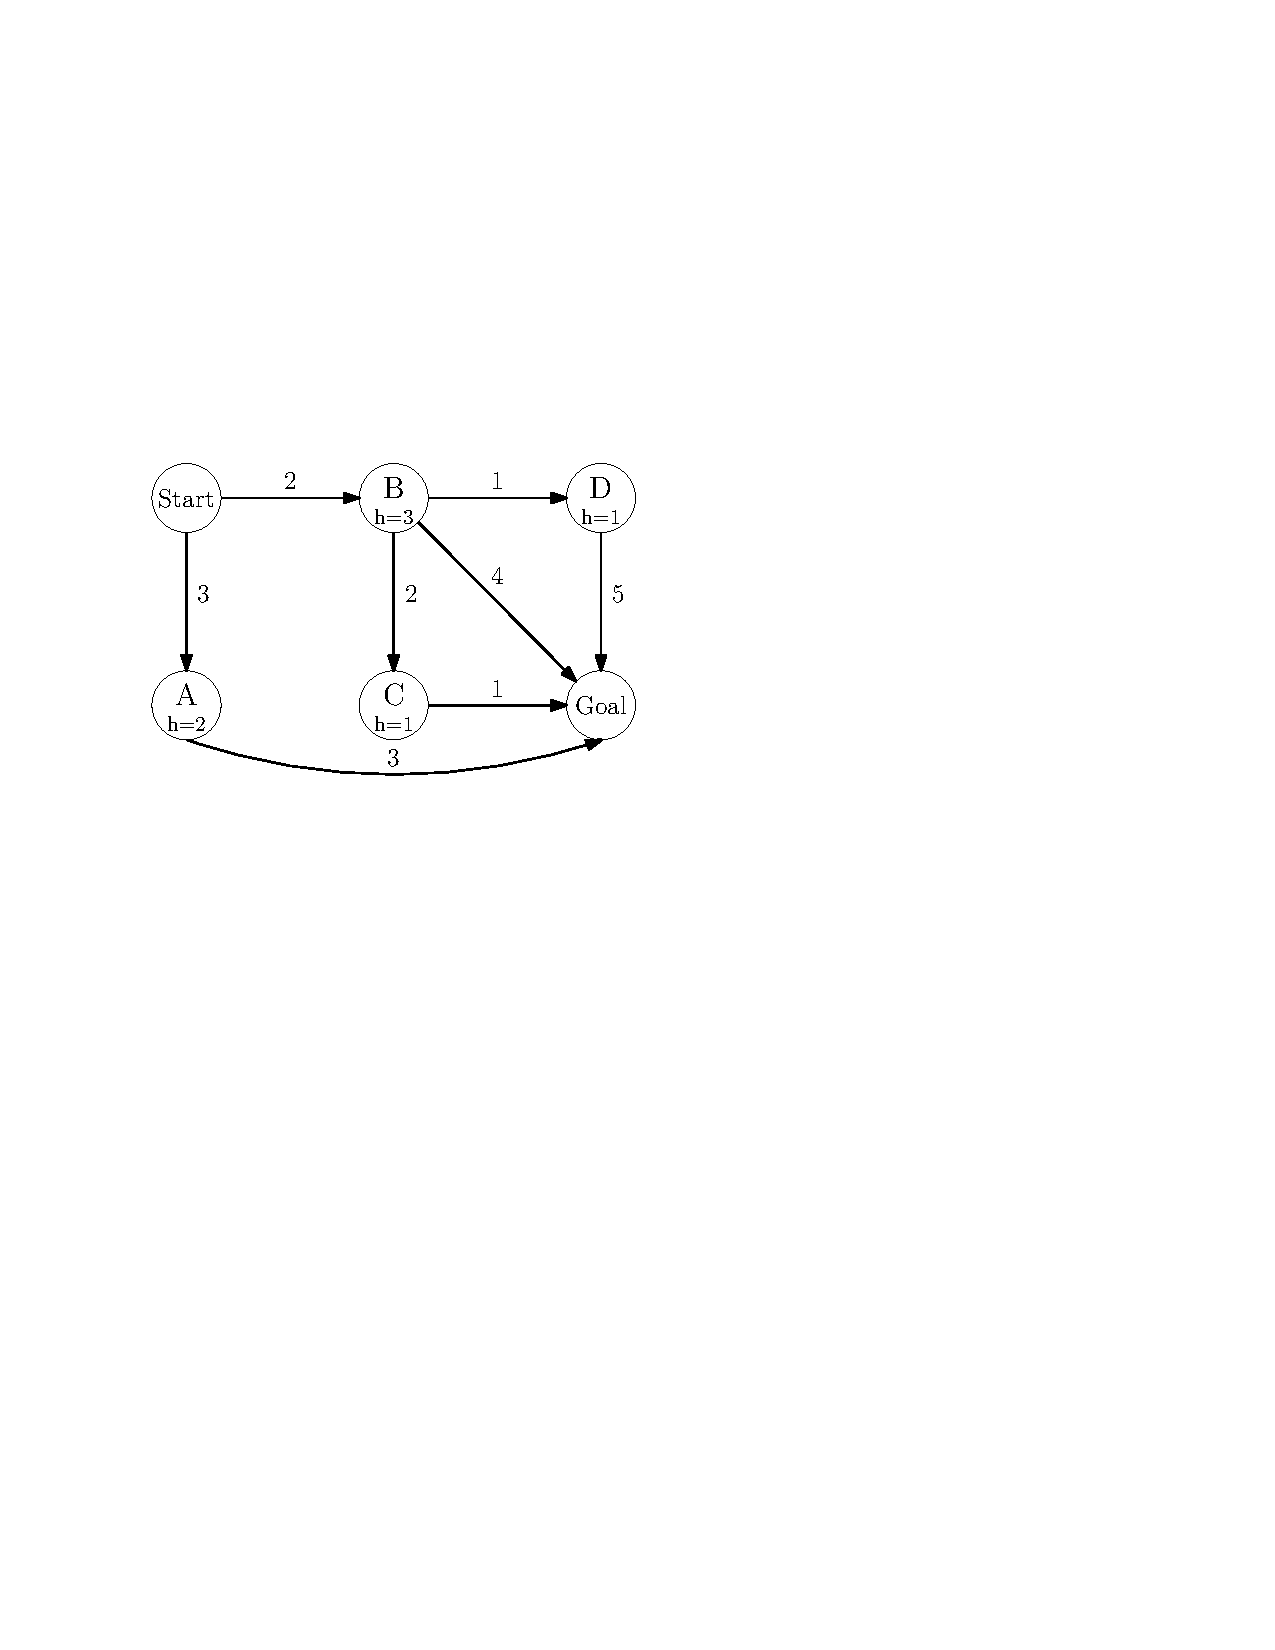
\includegraphics[width=0.5\textwidth]{hw1-statespace}

The available actions at each state are denoted by arrows with a path
cost label above each arrow.  For each of the following graph search
strategies, figure out the order in which states are expanded as well
as the path returned by graph search.  When choosing an arbitrary
order of state expansions (to break ties), use an alphabetical
ordering.  Remember that in graph search, states are expanded only
once.

% If you write your solution inline, feel free to comment out all of
% the problem definition above (especially the figure, which you
% probably won't have a copy of!).

\begin{enumerate}
\item Greedy search using the instantaneous transition costs
\item Depth first search
\item Breadth first search
\item Uniform cost search
\item Greedy search with the heuristic values listed at each state
\item A* search with the heuristic values listed at each state
\end{enumerate}

\newpage
\section{Downhill Skiing}

After getting to Alta, Alice takes the lift up to the top of the
mountain.  The run is really rocky, so her only option is to go
straight downhill.  She begins with a velocity of $0$ and can safely
maintain a maximum velocity of $V$.  At any state, she has three
actions she can take: accelerate, decelerate or coast.  If the
accelerates, her velocity increases by $1$; if she decelerates, it
decreases by $1$; if she coasts, it stays the same.  \emph{After} her
velocity is adjusted by her action, she moves downhill an equal number
of squares to her current velocity.

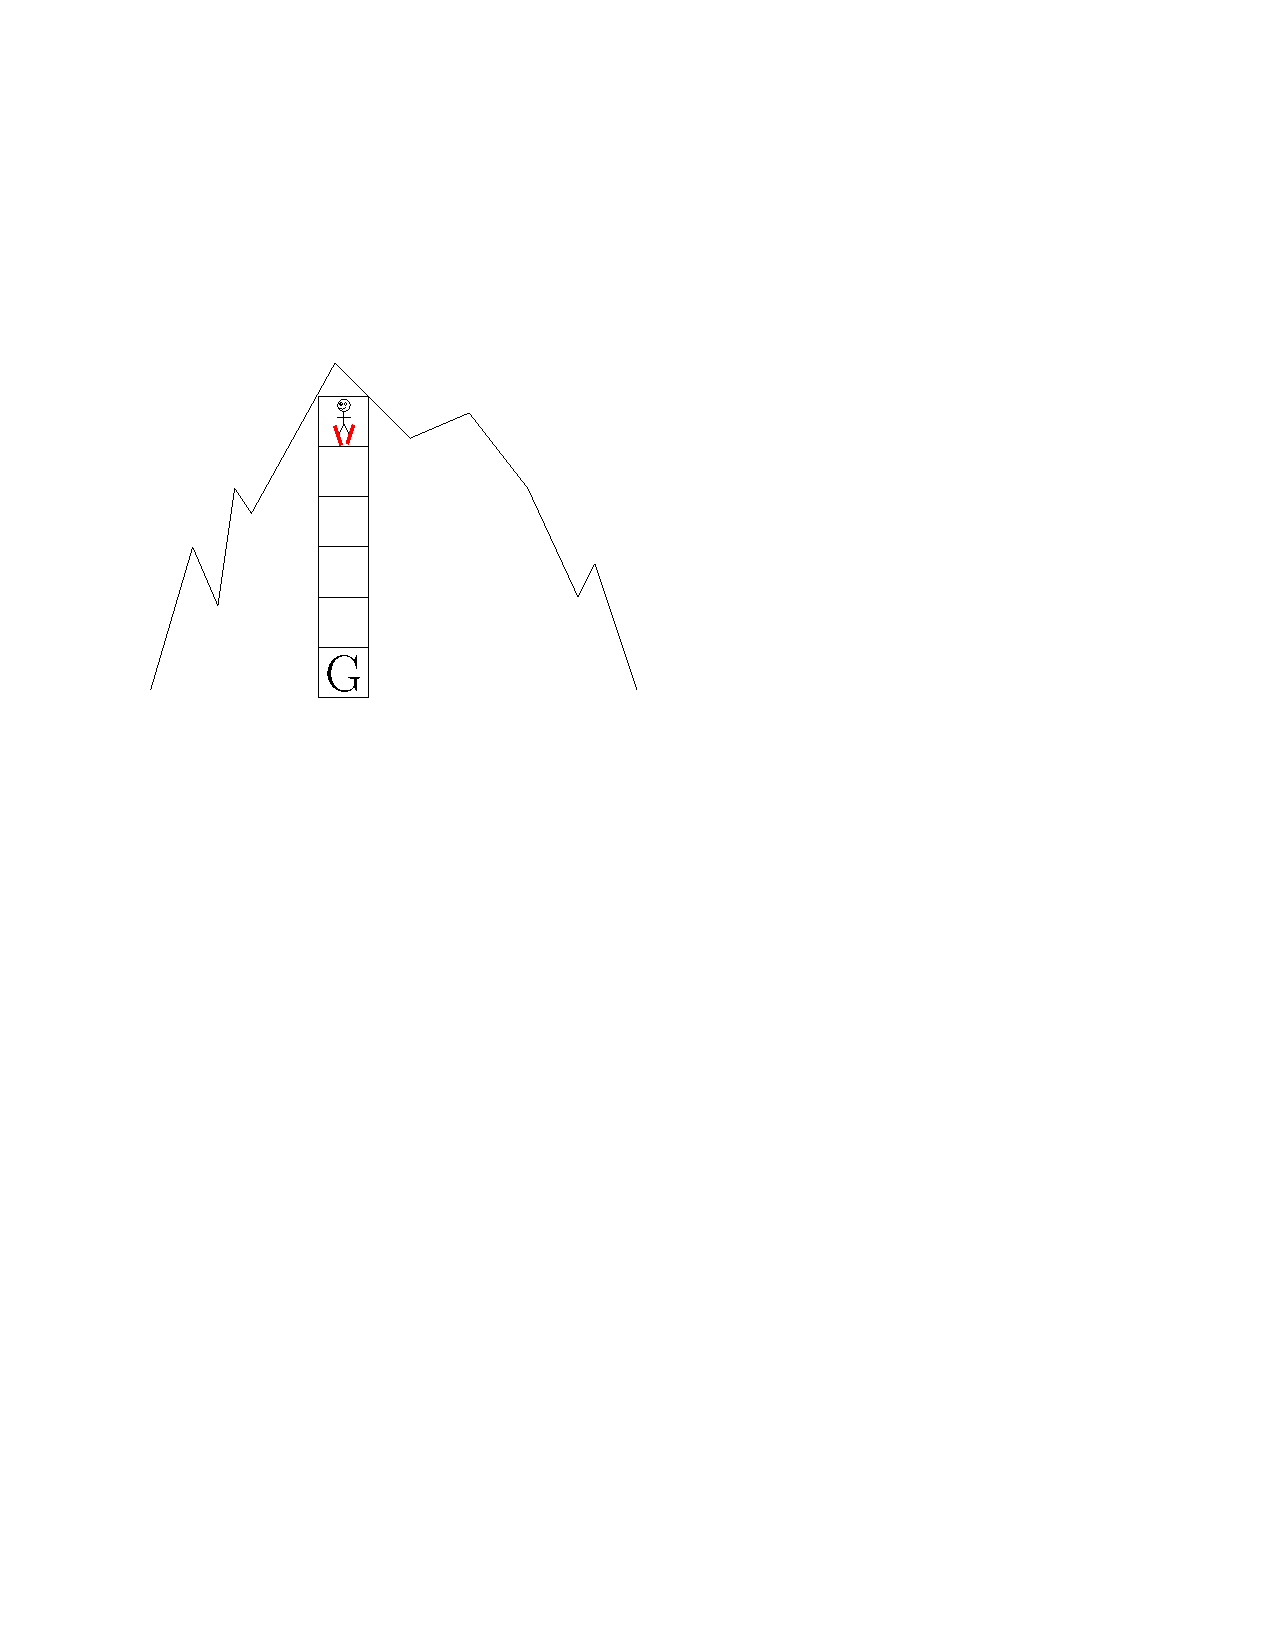
\includegraphics[width=0.5\textwidth]{hw1-skiing.pdf}

Consider the above figure.  If Alice's first action is ``accelerate''
then she will end up in the second square down with a velocity of
$1$.  If she then ``coasts'' then she will end up in the third square
down with a velocity of $1$.  If she ``accelerates'' again, she will
end up in the fifth square down with a velocity of $2$.

Alice's goal is to reach the chair lift (marked ``G'') with a velocity
of zero.  (No, Alice cannot have negative velocities).  She would like
to get there as quickly as possible.  However, if she has a non-zero
velocity at the goal, she skies into the parking lot and destroys her
skis.

% Ditto about commenting out the problem definition above.

\begin{enumerate}
\item If the mountain is $N$ units tall (eg., it is $N=6$ units tall in
the figure), what is the size of the state space?  Justify your
answer.  (You may ignore ``unreachable'' states.)  What are the
start/goal states?

\item Give an example of a state that is not reachable.  Suppose that
Alice cannot coast (she must either accelerate or decelerate): does this
yield \emph{more} unreachable states? If so, give an example of one and
justify your answer either way.

\item Is Alice's current elevation (i.e., distance from the chair lift)
an admissible heuristic?  Why or why not?

\item State and justify a non-trivial, admissible heuristic for this
problem which is \emph{not} current elevation.
\end{enumerate}

\end{document}

%%% Local Variables:
%%% mode: latex
%%% TeX-master: t
%%% End:
